\par\Needspace{14\baselineskip}
\section{多元函数的微分}
\label{sec:analysis-multivariable-differentiation}
\label{sec:multivariable-differentiation}

一元微分用一个斜率描述输入微调后的输出变化。对$f(x,y)=x^2+xy+y^2$，输入是二维点而输出仍是一个实数；若同一输入同时产生多个实数，才得到向量值函数。
下面先完整研究多元标量函数，再将线性近似推广到向量输出；矩阵自变量及局部方程的求解各自另作讨论。
这样，梯度始终对应标量输出，Jacobian矩阵始终记录多个输出分量的变化，二者的形状与作用不会混用。
向量、矩阵、迹与行列式沿用第~\ref{chap:sets-functions-and-proofs}章；极限与距离沿用第~\ref{chap:function-limits}章，连续、微分与勒贝格积分沿用第~\ref{chap:univariate-calculus}章的结论。
偏导数与局部线性近似可参考\scite{math-openstax-calculus3}，严格的多元微分论证可参考\scite{math-lebl2026analysis2}。

\subsection{多元标量函数的极限和连续性}
\label{sec:multivariable-limits-continuity}

本小节始终研究$f:D\subseteq\mathbb R^d\to\mathbb R$。多个输入坐标必须共同趋近一个点，输出误差则仍用实数绝对值度量。

\subsubsection{多元标量函数的定义}

固定一个坐标得到一元切片，恢复全部坐标后才是原来的多元函数。先明确输入与输出，才能区分“沿某个切片趋近”和“整个定义域中的趋近”。
\begin{definition}[多元标量函数]
\label{def:multivariable-scalar-function}
设$d$为正整数、$D\subseteq\mathbb R^d$。映射$f:D\to\mathbb R$称为多元标量函数；它把整个输入点$\bm x=(x_1,\ldots,x_d)^\top$映为一个实数$f(\bm x)$。
\end{definition}
例如$f(x,y)=x^2+xy+y^2$在$(1,2)$处取值$7$；固定$y=2$后得到的一元切片是$x\mapsto x^2+2x+4$，它只反映原函数在一条直线上的取值。

\subsubsection{极限的定义与判别}

在实轴上可以从左右两侧趋近，在平面中还可以沿直线、抛物线等路径趋近。
极限必须同时控制所有允许的输入，不能按路径分别选择互不兼容的误差范围。
\paragraph{极限的定义}
\label{sec:multivariable-joint-limits}

设$\bm D\subseteq\mathbb R^d$，$f:\bm D\to\mathbb R$，
$\bm a$是$\bm D$的聚点，即任意小的球内都有不同于$\bm a$的定义域点。
用欧氏距离$\lVert\bm x-\bm a\rVert_2$同时控制各坐标的偏移，便能把一元极限的邻域条件推广过来。
\begin{definition}[多元函数的极限]
\label{def:multivariable-limit}
若对每个$\varepsilon>0$，都存在$\delta>0$，使得
\[
 \bm x\in\bm D,\quad 0<\lVert\bm x-\bm a\rVert_2<\delta
 \quad\Longrightarrow\quad |f(\bm x)-L|<\varepsilon,
\]
则称$f$在$\bm x\to\bm a$时的极限为$L$，记为$\lim_{\bm x\to\bm a}f(\bm x)=L$。
\end{definition}
这里的同一个$\delta$必须控制球内全部允许输入。各坐标可以按不同速度趋近，
也可以让行进方向随位置改变。

\paragraph{序列判据与路径检验}
与一元情形一样，极限存在等价于：任意满足$\bm x_n\in\bm D\setminus\{\bm a\}$、
$\bm x_n\to\bm a$的序列都有$f(\bm x_n)\to L$。
这是第~\ref{sec:analysis-set-metric}节的一般度量空间序列判据在欧氏输入、实数输出下的应用，所需的输入与输出距离都已指定。
所以找到两条输出极限不同的路径足以否定极限，但验证有限条路径不能证明极限存在。

\begin{example}[坐标切片与所有直线仍会遗漏路径]
\label{ex:multivariable-path-limits}
令$f(0,0)=0$，非原点处令$f(x,y)=xy/(x^2+y^2)$。
沿两条坐标轴，函数都为$0$；沿$y=x$，函数恒为$1/2$，故原点处没有联合极限。
这个函数分别固定一个坐标后，在另一坐标上连续，但它在原点不联合连续。

即使验证所有过原点的直线，仍不足够。令$g(0,0)=0$，并在非原点处令
\[
 g(x,y)=\frac{x^2y}{x^4+y^2}.
\]
沿$y=kx$，当$k\neq0$时$g(x,kx)=kx/(x^2+k^2)\to0$；
当$k=0$或沿竖直轴时，函数为$0$。
可是沿抛物线$y=x^2$，$g(x,x^2)=1/2$。每条固定直线上的控制不能同时控制弯曲的趋近方式。
\end{example}


图~\ref{fig:analysis-process-joint-limit-paths}把直线路径和弯曲路径放到同一函数上，显示只检查直线可能遗漏的趋近方式。
\begin{figure*}[!htbp]
 \centering
 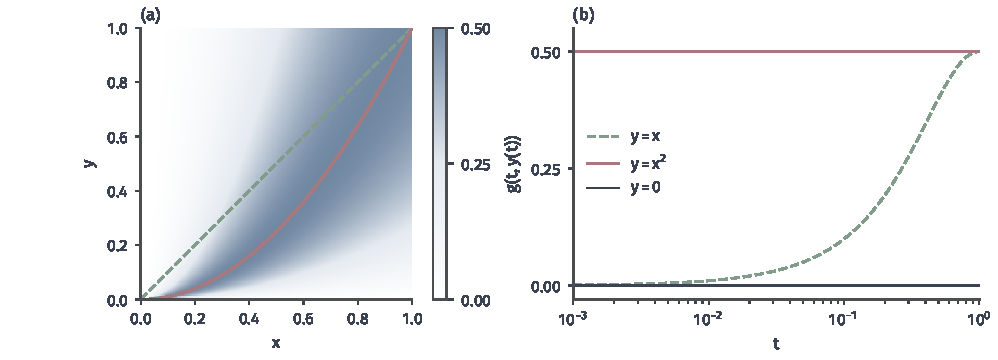
\includegraphics[width=169.0mm]{figures/01-mathematical-preliminaries-upper/01-mathematical-language-combinatorics-analysis-optimization/matplotlib/chapter3-concept-processes/joint-limit-paths.pdf}
 \caption{取前例$g(x,y)=x^2y/(x^4+y^2)$，原点另置零。(a) 第一象限的函数值及三条路径，色阶固定为$0$至$1/2$。(b) 沿$y=0$、$y=x$分别趋零，沿$y=x^2$恒为$1/2$；横轴为正参数$t$的对数刻度，向左趋近原点。不同路径极限足以否定联合极限，有限条路径不能反向证明存在。}
 \label{fig:analysis-process-joint-limit-paths}
\end{figure*}

\paragraph{累次极限与联合极限}
累次极限还会改变问题的量词。先令$y\to0$、再令$x\to0$，考察的是
$\lim_{x\to0}\lim_{y\to0}f(x,y)$，没有要求两个坐标同时趋近。
对上例的$f$，两个次序的累次极限都为$0$，联合极限却不存在。
又如$h(x,y)=x^2/(x^2+y^2)$在非原点定义，则
\[
 \lim_{x\to0}\lim_{y\to0}h(x,y)=1,
 \qquad
 \lim_{y\to0}\lim_{x\to0}h(x,y)=0.
\]
所以累次极限相等不是联合极限存在的充分条件；改变次序也可能改变累次极限。
如果联合极限存在，并且相关内层极限在去心邻域内存在，相应累次极限才必须等于联合极限。

\paragraph{统一误差估计}
要证明联合极限，可以寻找只依赖距离的统一上界。
例如$|xy|\leq(x^2+y^2)/2$，所以
\[
 \left|\frac{x^2y}{x^2+y^2}\right|
 \leq \frac{|x|}{2}
 \leq\frac12\sqrt{x^2+y^2}\longrightarrow0.
\]
这个估计同时覆盖全部路径，因此给出原点极限为$0$。极坐标也可用于估计，
但写成$(x,y)=(r\cos\theta,r\sin\theta)$后，仍需控制所有角度，不能只固定$\theta$再令$r\to0$。

\subsubsection{连续性的定义与运算}
\label{sec:multivariable-continuity}

连续性要求联合趋近时的输出恰好趋于基点值，形式与前面度量下的连续性相同。
这里先对全部输入作共同控制，再讨论运算后能否保留这种控制。
\begin{definition}[多元标量函数的连续性]
\label{def:multivariable-scalar-continuity}
设$f:D\subseteq\mathbb R^d\to\mathbb R$、$\bm a\in D$。若对每个$\varepsilon>0$都存在$\delta>0$，使
\[
 \bm x\in D,\quad\lVert\bm x-\bm a\rVert_2<\delta
 \Longrightarrow |f(\bm x)-f(\bm a)|<\varepsilon,
\]
则称$f$在$\bm a$处连续；在$D$上每点连续时称$f$为连续函数。
\end{definition}
聚点处这等价于联合极限等于$f(\bm a)$，孤立点处则自动成立。固定其他输入坐标后的一元切片连续只是必要条件，例~\ref{ex:multivariable-path-limits}说明它不足以保证联合连续。

\paragraph{和的连续性}
若$f,g$在$\bm a$处连续，则$f+g$也连续，因为和的输出误差不超过两个原误差之和。

\paragraph{差的连续性}
在相同条件下$f-g$连续：差的输出误差同样不超过两个原误差之和。

\paragraph{数乘的连续性}
若$f$在$\bm a$处连续，$c$为固定实数，则$cf$连续。$c\neq0$时将$f$的误差控制在$\varepsilon/|c|$以内即可；$c=0$时结论直接成立。

\paragraph{积的连续性}
若$f,g$在$\bm a$处连续，则$fg$连续。这由两个实数输出的积的极限法则得到。

\paragraph{商的连续性}
若$f,g$在$\bm a$处连续且$g(\bm a)\neq0$，则$g$在基点附近远离零，商的极限法则保证$f/g$连续。分母非零的条件不能省略。
多元多项式由连续坐标函数的有限运算得到，因此连续；分母非零处的有理函数同样连续。

\paragraph{标量复合函数}
若$f:D\to\mathbb R$在$\bm a$处连续，一元函数$\psi$在$f(\bm a)$处连续，且$f$的相邻输出在$\psi$的定义域内，则$\psi\circ f$连续。
先用$\psi$确定中间实数的允许误差，再由$f$控制输入点的欧氏距离，即得到复合函数的误差条件。

\subsubsection{一致连续性与闭有界集上的性质}

一致连续要求同一个输入误差尺度控制全部基点；有界性与最值存在则约束整个定义域上的函数值。
下面用有限维闭有界集内的收敛子列，分别说明这两类整体结论。

\paragraph{有限维闭有界集的收敛子列}
实数列的Bolzano--Weierstrass定理可以逐个坐标使用，得到多维输入所需的子列性质。
这里有界性负责产生收敛子列，闭性则进一步保留极限点。
\begin{theorem}[有限维有界序列的收敛子列]
\label{thm:multivariable-bolzano-weierstrass}
若$(\bm x_n)$是$\mathbb R^d$中的有界序列，则存在严格递增的正整数序列$(n_k)$及$\bm a\in\mathbb R^d$，使$\bm x_{n_k}\to\bm a$。
若所有$\bm x_n$属于闭集$K$，则$\bm a\in K$。
\end{theorem}
\begin{proof}
先用实数列定理选出第一坐标收敛的子列，再从这个子列中选出第二坐标收敛的子列，重复有限次后，全部坐标都收敛。
设各坐标极限组成$\bm a$，由$\lVert\bm x-\bm a\rVert_2\leq\sqrt d\max_j|x_j-a_j|$可知所得子列在欧氏距离下收敛。
若它属于闭集$K$，闭集包含其收敛序列的极限，故$\bm a\in K$。
\end{proof}
有限维闭有界集因此具有前面紧致性讨论中的子列性质，下面直接用它证明函数的整体性质。

\paragraph{一致连续性}
把连续定义中的$\delta$放在选择基点之前，就得到一致连续的要求。
具体地，对每个$\varepsilon>0$存在$\delta>0$，使所有$\bm x,\bm y\in D$满足$\lVert\bm x-\bm y\rVert_2<\delta$时都有$|f(\bm x)-f(\bm y)|<\varepsilon$。
闭有界集上的逐点连续足以给出这样的共同尺度。
\begin{theorem}[闭有界集上的一致连续性]
\label{thm:multivariable-uniform-continuity}
设$K\subseteq\mathbb R^d$非空、闭且有界，$f:K\to\mathbb R$连续，则$f$在$K$上一致连续。
\end{theorem}
\begin{proof}
定理~\ref{thm:analysis-uniform-continuity}的证明只用到定义域中任意点列都有域内收敛子列，以及连续性。
上一定理已为$K$建立这项子列性质；将输入距离改为欧氏范数，原证明便适用，无需重新构造反例点列。
\end{proof}
存在有限$L$使$|f(\bm x)-f(\bm y)|\leq L\lVert\bm x-\bm y\rVert_2$时，也直接得到一致连续；这是多元标量函数的Lipschitz条件。

\paragraph{有界性与极值达到}
要保证上、下确界由定义域内的点取得，还需要防止取值趋近确界的输入序列逃出定义域。
闭有界集的子列性质正好保留这种极限点。
\begin{theorem}[闭有界集上的极值定理]
\label{thm:multivariable-extreme-value}
设$K\subseteq\mathbb R^d$非空、闭且有界，$f:K\to\mathbb R$连续，则$f$有界，且存在$\bm x_{\min},\bm x_{\max}\in K$满足
\[
 f(\bm x_{\min})\leq f(\bm x)\leq f(\bm x_{\max})\qquad(\bm x\in K).
\]
\end{theorem}
\begin{proof}
定理~\ref{thm:analysis-extreme-value}已证明，定义域内的收敛子列性质与连续性共同保证有界及最值达到。
这里的$K$由定理~\ref{thm:multivariable-bolzano-weierstrass}满足同一子列条件，所以该证明适用，输出仍为实数。
\end{proof}
这些条件是充分保证。整个平面上的$f(x,y)=x^2+y^2$沿$y=0$退化为前面的实轴平方函数反例，所以连续却不一致连续。
在开单位圆盘上，同一函数的上确界为$1$却没有最大点，说明不能直接删去闭性。

\subsection{偏导数和梯度}

下面仍只研究实值函数$f:U\subseteq\mathbb R^d\to\mathbb R$，其中$U$为开集。先计算各坐标切片的变化率，再把这些标量排列为梯度；沿一般方向的变化率也在这里定义。

\subsubsection{偏导数}

开集保证基点附近足够小的双侧坐标扰动仍在定义域内。固定其他坐标后，就可以直接使用一元导数。
\begin{definition}[偏导数]
\label{def:multivariable-partial-derivative}
设$\bm a\in U$，令$\bm e_j$是第$j$个坐标为$1$、其余为$0$的向量。若双侧极限
\[
 \partial_jf(\bm a)=\frac{\partial f}{\partial x_j}(\bm a)
 =\lim_{t\to0}\frac{f(\bm a+t\bm e_j)-f(\bm a)}t
\]
存在且有限，就称它为$f$在$\bm a$处关于$x_j$的\term{偏导数}（partial derivative）。
\end{definition}
它表示只改变第$j$个坐标、其余坐标固定时的变化率。符号$\partial$提醒我们：这里求的是多元函数的一个坐标切片的导数。

例如对$f(x,y)=x^2+xy+y^2$，固定$y$求导得到$f_x=2x+y$；固定$x$得到$f_y=x+2y$。
在$(1,2)$处，两者为$4,5$。具体地，
\[
 \frac{f(1+t,2)-f(1,2)}t=4+t\longrightarrow4.
\]
这里$f_x(1,2)=4$并不意味着同时改变$x,y$时都以斜率$4$变化。每一个偏导数只说明自己的坐标切片。

\subsubsection{梯度}

各偏导数采用相同的基点，但分别对应不同输入坐标。将这些变化率按坐标顺序排列，就能用一个向量记录所有坐标切片的信息。
\begin{definition}[梯度]
\label{def:multivariable-gradient}
若$f:U\to\mathbb R$在$\bm a$处的各一阶偏导数都存在，称列向量
\[
 \nabla f(\bm a)=\bigl(\partial_1f(\bm a),\ldots,\partial_df(\bm a)\bigr)^\top
\]
为$f$在$\bm a$处的\term{梯度}（gradient）。
\end{definition}
对$f(x,y)=x^2+xy+y^2$，有$\nabla f(x,y)=(2x+y,x+2y)^\top$，所以$\nabla f(1,2)=(4,5)^\top$。
梯度的存在只说明各偏导数存在，尚未保证它能预测所有坐标同时改变时的函数增量；这要由后面的可微性判断。

\subsubsection{方向导数}

沿坐标轴求导只是方向变化的一部分。若让多个坐标按一个固定向量共同移动，就得到另一条一元切片。
\begin{definition}[方向导数]
\label{def:multivariable-directional-derivative}
给定向量$\bm v\in\mathbb R^d$，若双侧极限
\[
 D_{\bm v}f(\bm a)
 =\lim_{t\to0}\frac{f(\bm a+t\bm v)-f(\bm a)}t
\]
存在且有限，就称它为沿$\bm v$的\term{方向导数}（directional derivative）。
\end{definition}
本书允许$\bm v$不是单位向量，导数按参数$t$的变化计量；若要表示每单位路程的变化率，应取$\lVert\bm v\rVert_2=1$。
取$\bm v=\bm e_j$便回到偏导数。双侧极限与只令$t\downarrow0$的单侧方向导数要分别判断。

仍取上述$f$，从$(1,2)$沿$\bm v=(1,1)^\top$移动，有
\[
 f(1+t,2+t)=7+9t+3t^2,
 \qquad D_{(1,1)}f(1,2)=9.
\]
改用同向单位向量$\bm u=(1,1)^\top/\sqrt2$，变化率为$9/\sqrt2$。
两者描述同一条直线，但参数速度不同，不能忽略归一化约定。

\subsection{多元标量函数的可微性}
\label{sec:multivariable-total-differentiation}

偏导数和方向导数分别检查固定的坐标轴或直线。若要同时控制任意小扰动，包括方向不断改变的扰动，就需要一个共同的线性近似。

\subsubsection{微分的定义}

预测增量应与扰动的叠加和数乘相容，因此使用线性映射$A:\mathbb R^d\to\mathbb R$。
例如$A(\bm h)=\bm c^\top\bm h$把每个坐标的扰动乘以固定系数再相加；可微性还要求遗漏的误差比扰动长度更小。
\begin{definition}[多元标量函数的可微性与全微分]
\label{def:multivariable-total-differential}
设$U\subseteq\mathbb R^d$开，$f:U\to\mathbb R$，$\bm a\in U$。
若存在一个线性映射$A:\mathbb R^d\to\mathbb R$，使
\begin{equation}
 f(\bm a+\bm h)=f(\bm a)+A(\bm h)+o(\lVert\bm h\rVert_2),
 \qquad\bm h\to\bm0,
\label{eq:analysis-total-differentiability}
\end{equation}
则称$f$在$\bm a$处\term{可微}（differentiable）。线性映射$A$称为该点的\term{全微分}（total differential），记为$\mathrm df_{\bm a}$。
\end{definition}
余项条件是$|f(\bm a+\bm h)-f(\bm a)-A(\bm h)|/\lVert\bm h\rVert_2\to0$。
它要求一个$A$适用于全部趋零扰动，并非先固定一个方向再允许误差控制随方向改变。

\subsubsection{可微性的要求与判别}
\label{sec:analysis-differentiability-relations}

固定开集$U\subseteq\mathbb R^d$、标量函数$f:U\to\mathbb R$与基点$\bm a\in U$。
下面先说明统一线性近似必然满足哪些要求，再给出可核查的充分判别，最后结合蕴含关系与反例，区分偏导数存在、全部双侧方向导数存在、可微和连续可微。

\paragraph{可微的必要条件}
若同一个线性近似有效，它在线性切片上必须与一元导数相同，函数增量本身也必须趋零。
这就把全微分与前面定义的偏导数、梯度及方向导数联系起来。
\begin{theorem}[可微性与梯度、方向导数]
\label{thm:multivariable-differentiable-necessary}
若$f:U\to\mathbb R$在$\bm a$处可微，则$f$在该点连续，各偏导数存在，并且
\[
 \mathrm df_{\bm a}(\bm h)=\nabla f(\bm a)^\top\bm h,
 \qquad D_{\bm v}f(\bm a)=\nabla f(\bm a)^\top\bm v
 \quad(\bm v\in\mathbb R^d).
\]
\end{theorem}
\begin{proof}
线性性给出$A(\bm h)=\sum_jh_jA(\bm e_j)$。由有限和的Cauchy--Schwarz不等式，
\[
 |A(\bm h)|\leq\left(\sum_j|A(\bm e_j)|^2\right)^{1/2}\lVert\bm h\rVert_2.
\]
因此线性项与余项都随$\bm h\to0$而趋零，得到$f$连续。
分别取$\bm h=t\bm e_j$并除以$t$，可知$\partial_jf(\bm a)=A(\bm e_j)$；线性性给出$A(\bm h)=\sum_j\partial_jf(\bm a)h_j$。
再对固定$\bm v$取$\bm h=t\bm v$，余项除以$t$仍趋零，就得到方向导数公式；$\bm v=\bm0$时差商恒为零。
\end{proof}
\begin{example}[二元二次函数的全微分]
\label{ex:multivariable-quadratic-differential}
对二次函数$f(x,y)=x^2+xy+y^2$，在$(1,2)$处有$\nabla f=(4,5)^\top$。设扰动为$(h,k)$，直接展开得
\[
 f(1+h,2+k)=7+4h+5k+(h^2+hk+k^2).
\]
由$|hk|\leq(h^2+k^2)/2$，最后一项绝对值不超过$3(h^2+k^2)/2$。除以$\sqrt{h^2+k^2}$后趋于零，所以全微分确为$4h+5k$。它同时解释了两个偏导数和沿$(1,1)$的变化率$4+5=9$。
\end{example}


图~\ref{fig:analysis-process-total-differential-remainder}将这个全微分的切平面与统一余项界对应起来。
\begin{figure*}[!htbp]
 \centering
 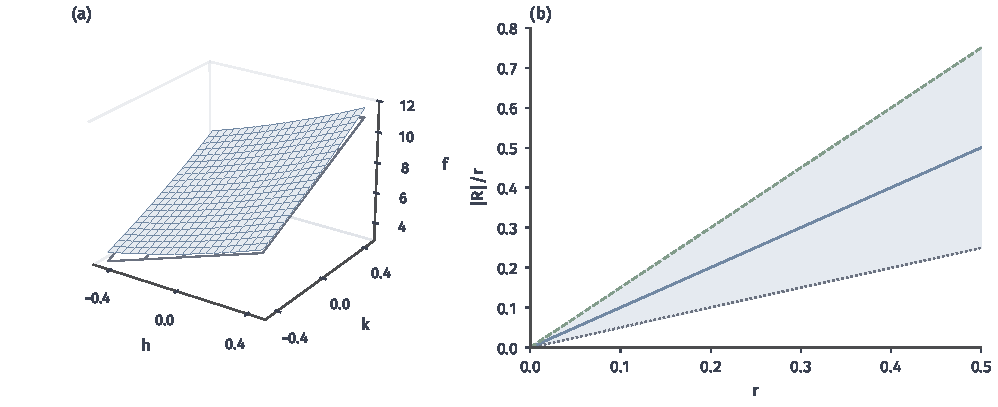
\includegraphics[width=169.0mm]{figures/01-mathematical-preliminaries-upper/01-mathematical-language-combinatorics-analysis-optimization/matplotlib/chapter3-concept-processes/total-differential-remainder.pdf}
 \caption{对二次函数在$(1,2)$处，灰网格是$P=7+4h+5k$，蓝面是$f(1+h,2+k)$。(b) 令$r=\sqrt{h^2+k^2}$，余项$R=h^2+hk+k^2$满足$r/2\leq R/r\leq3r/2$；阴影给出所有方向的完整范围，三条线是其中的代表值。共同上界随$r\to0$趋零，才保证任意方向都适用同一个线性近似。}
 \label{fig:analysis-process-total-differential-remainder}
\end{figure*}

对单位方向$\bm u$，内积不等式给出$D_{\bm u}f(\bm a)\leq\lVert\nabla f(\bm a)\rVert_2$。
当梯度非零时，在$\bm u=\nabla f(\bm a)/\lVert\nabla f(\bm a)\rVert_2$处取等号，故可微函数的梯度方向是局部上升最快的单位方向。
这个结论需要可微性，不能只由梯度向量存在推出。


图~\ref{fig:analysis-process-gradient-level-curves}用同一个二次函数比较梯度方向、等值曲线切向及另一个单位方向。
\begin{figure}[!htbp]
 \centering
 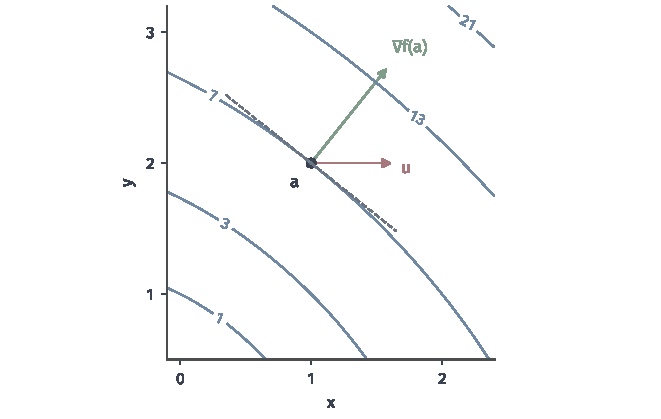
\includegraphics[width=112.0mm]{figures/01-mathematical-preliminaries-upper/01-mathematical-language-combinatorics-analysis-optimization/matplotlib/chapter3-concept-processes/gradient-level-curves.pdf}
 \caption{$f=x^2+xy+y^2$的等值曲线，标注为函数值；基点$a=(1,2)$处$\nabla f=(4,5)^\top$，图中绿箭头按$0.15$倍绘制。灰虚线沿$(5,-4)^\top$，与梯度垂直，因而与经过$a$的等值曲线相切；红箭头为$u=(1,0)^\top$。比较最快上升方向时须先归一化，不能直接比较图中箭头长度。}
 \label{fig:analysis-process-gradient-level-curves}
\end{figure}

\paragraph{偏导数连续给出的充分条件}
如果各坐标的变化率在同一点附近连续，就可以用它们共同控制全部坐标增量。
与上面的必要条件不同，这项条件可以直接保证全微分存在。
\begin{theorem}[偏导数连续与可微性]
\label{thm:multivariable-continuous-partials-sufficient}
设$f:U\to\mathbb R$，$U$开，$\bm a\in U$。若各一阶偏导数在$\bm a$的某个邻域内存在，并在$\bm a$处连续，则$f$在$\bm a$处可微。
\end{theorem}
\begin{proof}
这项条件可以沿坐标逐个改变来核对：把$\bm a$到$\bm a+\bm h$的增量拆成$d$段，
每段只改一个坐标，一元中值定理将该段增量写成相应中间点处的偏导数乘$h_j$。
当$\bm h\to\bm0$时，所有中间点都趋于$\bm a$；偏导连续性因此使
\[
 \begin{aligned}
 &\left|f(\bm a+\bm h)-f(\bm a)-\sum_{j=1}^d\partial_j f(\bm a)h_j\right|\\
 &\qquad\leq \max_j\left|\partial_j f(\bm\xi_j)-\partial_j f(\bm a)\right|
       \sum_{j=1}^d|h_j|
 =o(\lVert\bm h\rVert_2),
 \end{aligned}
\]
其中$\bm\xi_j$是第$j$段的中间点，最后一步用了$\sum_j|h_j|\leq\sqrt d\lVert\bm h\rVert_2$。
这就把各坐标上的变化拼成了同一个有效的全微分。
\end{proof}
偏导数连续只是充分条件。可微仅要求函数增量具有统一的一阶近似，不要求这些系数随基点连续变化。

\paragraph{连续可微函数}
若还希望各点的一阶系数连续变化，就需在一个范围内同时控制偏导数。
实值函数的各一阶偏导数在开集$U$上存在且连续时，称它在$U$上连续可微，记为$C^1(U)$；$C^k(U)$表示直至$k$阶的各偏导数都存在且连续。
刚才的充分条件保证$C^1$函数处处可微，逆向并不成立。

\paragraph{条件之间的蕴含关系}
由必要条件与充分判别，现在可以把这些要求放在一起比较：
\[
 \begin{gathered}
 f\text{在}\bm a\text{的某邻域内连续可微}
 \ \Longrightarrow\ f\text{在}\bm a\text{处可微},\\
 f\text{在}\bm a\text{处可微}
 \ \Longrightarrow\ \text{全部双侧方向导数存在}
 \ \Longrightarrow\ \text{全部偏导数存在}.
 \end{gathered}
\]
第一条已由连续偏导数的充分判别得到，第二条已由必要条件定理证明，最后只须在全部方向中取坐标方向$\bm e_j$。
可微还蕴含连续，并使方向导数关于方向成为同一个线性映射；相应公式已在必要条件中给出。
首项要求一个邻域内偏导数连续，其余各项只约束同一基点；即使要求处处可微，也不能反推连续可微。
一元函数的普通导数存在就等价于可微，多元函数则还须协调多个输入方向，所以上面各条逆命题需要分别检验。

\paragraph{偏导数存在不保证可微}
下面检验蕴含链中的逆命题。先看坐标偏导数：它们只约束坐标切片，并未控制其余方向或路径。
\begin{example}[偏导数存在但不可微]
\label{ex:analysis-partials-not-differentiable}
定义$f:\mathbb{R}^2\to\mathbb{R}$为
\[   f(x,y)=
\begin{cases}     \dfrac{xy}{\sqrt{x^2+y^2}}, & (x,y)\neq(0,0),\\[6pt]     0, & (x,y)=(0,0).
\end{cases} \]
沿两条坐标轴，函数恒为$0$，所以 $\partial f/\partial x(0,0)=\partial f/\partial y(0,0)=0$。若$f$在原点可微， 候选线性部分只能是零映射。可是沿$\bm{h}=(t,t)$，
\[   \frac{|f(t,t)-f(0,0)|}{\lVert(t,t)\rVert_2}   =   \frac{|t|/\sqrt{2}}{\sqrt{2}|t|}   =\frac12, \]
余项与$\lVert\bm{h}\rVert_2$之比不趋于零，故$f$在原点不可微。偏导数只看坐标轴，遗漏了其他接近路径。本例沿每个方向$\bm v=(a,b)$的
正向方向导数都存在，这里只令$t\downarrow0$，得到$ab/\sqrt{a^2+b^2}$（零方向取$0$）；它却不是关于$\bm v$
的线性函数，而且双侧方向导数在$ab\neq0$时不存在。方向极限采用单侧还是双侧，
必须与所用定义一致；本节定义采用双侧极限。
本例还在原点连续，因为$|xy|/\sqrt{x^2+y^2}\leq\sqrt{x^2+y^2}/2$；所以补上连续性也不能反推可微。
\end{example}

\paragraph{全部方向导数存在不保证可微}
从坐标切片扩展到所有固定直线，仍需检查这些变化率能否组成线性映射，以及是否具有统一余项。先看缺少线性性的情形，令
$g(x,y)=x^3/(x^2+y^2)$于非零点，$g(0,0)=0$。
沿$\bm v=(a,b)\neq\bm0$有$D_{\bm v}g(0,0)=a^3/(a^2+b^2)$，
但坐标方向导数给出的候选梯度为$(1,0)^\top$，它对方向$(1,1)^\top$
预测$1$而非实际的$1/2$。这些方向变化率无法拼成一个线性映射。
与前例的单侧方向极限相比，这里直接检验了本节采用的双侧定义。

\begin{example}[所有方向导数为零仍不足以可微]
\label{ex:multivariable-linear-directionals-not-differentiable}
前面的双侧方向导数反例不能组成线性函数。即使补上这一要求，仍需检查统一余项。
在非原点处令$q(x,y)=x^3y/(x^4+y^2)$，并令$q(0,0)=0$。
由$2|x^2y|\leq x^4+y^2$，有$|q(x,y)|\leq|x|/2$，故$q$在原点连续。
对固定方向$(a,b)^\top$，若$b\neq0$，
\[
 \frac{q(ta,tb)}t=\frac{t a^3b}{t^2a^4+b^2}\longrightarrow0;
\]
若$b=0$，差商恒为零。因此所有双侧方向导数都为零，它们也组成零线性映射。
可是沿$\bm h=(t,t^2)^\top$，$q(t,t^2)=t/2$，从而
\[
 \frac{|q(t,t^2)|}{\lVert(t,t^2)\rVert_2}
 =\frac1{2\sqrt{1+t^2}}\longrightarrow\frac12.
\]
候选零映射不能满足全微分的余项条件。方向导数先固定方向再取极限，
全微分则要求对方向随扰动改变的序列也有同一个误差控制。
\end{example}

\paragraph{可微不保证连续可微}
一元函数已经足以否定这个逆命题。在实轴上令$r(0)=0$，$x\neq0$时令$r(x)=x^2\sin(1/x^2)$。
由于$r(h)/h=h\sin(1/h^2)\to0$，有$r'(0)=0$；非零点按运算法则求导得到
\[
 r'(x)=2x\sin(1/x^2)-\frac{2}{x}\cos(1/x^2).
\]
取$x_n=(2\pi n)^{-1/2}$，有$r'(x_n)=-2/x_n\to-\infty$，所以$r'$在$0$处不连续，$r$却处处可微。
在多元情形令$f(\bm x)=r(x_1)$，同样得到处处可微而非连续可微的标量函数。
这个例子还说明可微不保证局部Lipschitz：若原点邻域内有共同Lipschitz常数，那里每个已存在的一元导数都应被这个常数控制，与上述无界导数矛盾。

\paragraph{连续不保证偏导数存在}
反方向也不能从连续性补回微分条件。
例如$f(x,y)=|x|$在整个平面上Lipschitz连续，但原点关于$x$的双侧偏导数不存在，因此在那里不可微。
反向也失败：例~\ref{ex:multivariable-path-limits}中原点置零的$xy/(x^2+y^2)$沿坐标轴恒零，两个偏导数存在，但原点不连续。
因此连续与偏导数存在之间没有一般单向蕴含；可微则能够同时保证二者。

\paragraph{梯度与线性近似的使用条件}
上述反例区分了两种用途：仅有偏导数时，梯度只是坐标变化率排成的向量；确认可微以后，才可用它统一预测增量，并用内积计算任意方向导数。
连续偏导数提供方便的充分判别，却不是必要条件；不满足该判别时，应回到全微分的统一余项定义检查。
后面讨论向量值函数时，将对各个标量输出分量分别检查，再组成Jacobian及复合微分。

\subsubsection{微分的运算法则}

以下$f,g$都在同一开集内定义，并在基点$\bm a$处可微，$c$为固定实数。
将各自的一阶展开相加或相乘，比较线性项与高阶余项，就能逐项得到下面的法则。

\paragraph{和的微分}
函数相加时，一阶近似相加，因此
\[
 \mathrm d(f+g)=\mathrm df+\mathrm dg.
\]
右侧微分在同一基点作用于同一个扰动，两个$o(\lVert\bm h\rVert_2)$余项相加后仍满足可微性要求。

\paragraph{差的微分}
函数相减时，一阶近似相减，因此
\[
 \mathrm d(f-g)=\mathrm df-\mathrm dg.
\]
余项之差仍为$o(\lVert\bm h\rVert_2)$，所以差函数也可微。

\paragraph{数乘的微分}
固定系数只会缩放线性项与余项，故$\mathrm d(cf)=c\,\mathrm df$，包括$c=0$的常函数情形。

\paragraph{积的微分}
展开$(f(\bm a)+\mathrm df(\bm h)+o(\lVert\bm h\rVert_2))(g(\bm a)+\mathrm dg(\bm h)+o(\lVert\bm h\rVert_2))$，保留一次项，得到
\[
 \mathrm d(fg)=g(\bm a)\,\mathrm df+f(\bm a)\,\mathrm dg.
\]
两个线性增量的乘积为$O(\lVert\bm h\rVert_2^2)$，可并入一阶余项，故该计算确实证明乘积可微。

\paragraph{商的微分}
若$g(\bm a)\neq0$，连续性保证邻近分母远离零。一元倒数函数的展开给出$\mathrm d(1/g)=-\mathrm dg/g(\bm a)^2$，再用积法则得到
\[
 \mathrm d(f/g)=\frac{g(\bm a)\,\mathrm df-f(\bm a)\,\mathrm dg}{g(\bm a)^2}.
\]
这里分母非零是定义商函数及估计余项的共同条件。

\paragraph{标量复合函数的微分}
若一元函数$\psi$在$f(\bm a)$处可微，且复合在邻域内有定义，将$f$的增量代入$\psi$的一元展开得到
\[
 \mathrm d(\psi\circ f)=\psi'(f(\bm a))\,\mathrm df.
\]
因为$f(\bm a+\bm h)-f(\bm a)=O(\lVert\bm h\rVert_2)$，外层的一阶余项仍是$o(\lVert\bm h\rVert_2)$。

\paragraph{二次型的微分}
向量自变量的二次型仍是标量函数，有限和的乘积法则可以直接用于它。考虑$q(\bm{x})=\bm{x}^{\top}\bm{A}\bm{x}$，其中 $\bm{A}\in\mathbb{R}^{d\times d}$固定。由乘积法则，
\begin{align*}
  \mathrm{d}q
  &=
  (\mathrm{d}\bm{x})^{\top}\bm{A}\bm{x}
  +\bm{x}^{\top}\bm{A}\,\mathrm{d}\bm{x}\\
  &=
  \bm{x}^{\top}(\bm{A}^{\top}+\bm{A})\,\mathrm{d}\bm{x}.
\end{align*}
因此
\begin{equation}
  \nabla_{\bm{x}}
  \bigl(\bm{x}^{\top}\bm{A}\bm{x}\bigr)
  =
  (\bm{A}+\bm{A}^{\top})\bm{x}.
\label{eq:analysis-quadratic-form-gradient}
\end{equation}
只有当$\bm{A}$对称时才能化为$2\bm{A}\bm{x}$。直接写成$2\bm{A}\bm{x}$会悄然加入对称性条件。

\subsubsection{中值定理与Lipschitz条件}

导数控制一点处的变化；若连接两点的整条线段都在定义域内，可以沿线段使用一元中值定理，得到有限增量的结论。
\begin{theorem}[多元标量函数的中值公式]
\label{thm:multivariable-scalar-mean-value}
设$f$在包含$[\bm x,\bm y]$的开集上可微，$\bm x\neq\bm y$。则存在$\theta\in(0,1)$使
\[
 f(\bm y)-f(\bm x)=\nabla f(\bm x+\theta(\bm y-\bm x))^\top(\bm y-\bm x).
\]
特别地，若沿线段有$\lVert\nabla f\rVert_2\leq L$，则$|f(\bm y)-f(\bm x)|\leq L\lVert\bm y-\bm x\rVert_2$。
\end{theorem}
\begin{proof}
令$\phi(t)=f(\bm x+t(\bm y-\bm x))$。由方向导数公式，$\phi'(t)=\nabla f(\bm x+t(\bm y-\bm x))^\top(\bm y-\bm x)$。
对$\phi$使用一元中值定理得到等式，再用内积不等式得到增量界。
\end{proof}
如果定义域是凸开集且各点梯度范数都不超过同一个有限$L$，任意两点间的线段都在域内，故$f$在全域满足Lipschitz条件。
局部邻域上有这样的界时得到局部Lipschitz条件；不能忽略连接线段是否属于定义域。

特别地，若$f\in C^1(U)$，在每个基点附近取一个包含在$U$内的闭球，连续梯度在球上有界，球内线段也不离开球，故上述估计保证$f$局部Lipschitz。
这不自动给出全域共同常数：实轴上的$x^2$连续可微，但其梯度在全域无界，因而不是全域Lipschitz函数。

\subsection{多元标量函数的高阶微分}
\label{sec:multivariable-curvature-error}

一阶微分记录局部线性变化，高阶微分进一步说明这些系数怎样变化。
下面先把二阶偏导数集中为Hessian矩阵，再用Taylor公式建立二阶近似，最后据此判断驻点的局部极值类型。

\subsubsection{二阶偏导数与Hessian矩阵}

一阶偏导数本身仍是多元标量函数，可以再次求偏导。这里记$f_{x_i x_j}=\partial_j(\partial_i f)$，即先对$x_i$、再对$x_j$求导。
对$f(x,y)=x^2+xy+y^2$，有$f_{xx}=2$、$f_{xy}=f_{yx}=1$、$f_{yy}=2$。一般函数的混合偏导数能否交换，需要额外条件。

\paragraph{混合偏导数的交换}
分别沿两个坐标求导时，先后次序未必自动无关。下面的连续性条件可以把两种次序联系起来。
\begin{theorem}[混合偏导数的交换]
\label{thm:multivariable-mixed-partials}
设$f$在$\bm a$的某个开邻域内有一阶偏导数$\partial_i f,\partial_j f$，混合偏导数$\partial_j\partial_i f,\partial_i\partial_j f$在该邻域存在并在$\bm a$处连续，则
\[
 \partial_j\partial_i f(\bm a)=\partial_i\partial_j f(\bm a).
\]
特别地，$C^2$函数的混合偏导数处处可以交换。
\end{theorem}
\begin{proof}
固定其他坐标，只需讨论二元函数在$(a,b)$处的情形。对小的非零$h,k$考察二阶差分
\[
 \Delta(h,k)=f(a+h,b+k)-f(a+h,b)-f(a,b+k)+f(a,b).
\]
令$\phi(x)=f(x,b+k)-f(x,b)$。先对$\phi$用一元中值定理，再对$y\mapsto f_x(\xi,y)$使用一次中值定理，得到
\[
 \Delta=h[f_x(\xi,b+k)-f_x(\xi,b)]=hk f_{xy}(\xi,\eta),
\]
其中$\xi$在$a,a+h$之间、$\eta$在$b,b+k$之间。先沿$y$方向拆分则得到$\Delta=hk f_{yx}(\xi',\eta')$。
除以$hk$后令$h,k\to0$，各中间点趋于$(a,b)$，连续性使两种混合偏导数在该点相等。
\end{proof}
只有偏导数存在而没有这些连续性条件时，结论可能失败。

\paragraph{Hessian矩阵}
把各偏导数的坐标变化率集中起来，就得到记录二阶信息的矩阵。
它的行、列分别对应先后两次求导的输入坐标。
\begin{definition}[Hessian矩阵]
\label{def:multivariable-hessian}
若$f:U\to\mathbb R$在$\bm x$附近有一阶偏导数，且各$\partial_j\partial_i f(\bm x)$存在，则称
\[
 \nabla^2f(\bm x)=\bigl[\partial_j\partial_i f(\bm x)\bigr]_{i,j=1}^d
\]
为$f$在该点的\term{Hessian矩阵}（Hessian matrix）。
\end{definition}
二阶偏导数存在本身尚不保证一阶导数具有统一的线性近似；二阶可微要求一阶导数映射本身可微。
$C^2$是保证二阶可微的充分条件，且此时Hessian对称。对上面的二次函数，Hessian就是$\begin{bmatrix}2&1\\1&2\end{bmatrix}$。
若$f\in C^2$，沿直线$t\mapsto f(\bm x+t\bm v)$求两次导数，在$t=0$处得到
\[
 \bm v^\top\nabla^2f(\bm x)\bm v
 =\sum_{i=1}^d\sum_{j=1}^d \partial_j\partial_i f(\bm x)v_i v_j.
\]
这个实数二次型衡量沿给定方向的一阶斜率变化。

对二次函数
\[   f(\bm{x})   =   \frac12\bm{x}^{\top}\bm{A}\bm{x}   +\bm{b}^{\top}\bm{x}+c, \]
只有$\bm{A}$的对称部分影响函数值。令 $\bm{H}=(\bm{A}+\bm{A}^{\top})/2$，则 $\nabla f(\bm{x})=\bm{H}\bm{x}+\bm{b}$且 $\nabla^2f(\bm{x})=\bm{H}$。
例如$\bm H=\operatorname{diag}(2,100)$时，方向二次型为$2v_1^2+100v_2^2$，
沿两个坐标方向都向上弯，但第二个方向的二阶变化率是第一个的$50$倍。
若改为$\operatorname{diag}(2,-100)$，两个坐标方向的弯曲方向便相反。
判断曲率需要检查整个二次型，而不是某一个对角元素。

对实对称矩阵$\bm H$，若每个非零$\bm v$都有$\bm v^\top\bm H\bm v>0$，称$\bm H$正定；
若只要求$\bm v^\top\bm H\bm v\geq0$，则称半正定。
把不等号反向得到负定与半负定；若既存在使二次型为正的方向，又存在使它为负的方向，
则称矩阵不定。这些名称分别说明全部方向或某些方向上的曲率符号。



\subsubsection{Taylor公式与局部近似}

把多个坐标同时改变的位移写成一条线段上的参数变化，就能回用一元Taylor公式。
下述公式都针对标量输出，二阶项是一个实数二次型。

一元Taylor定理可沿整条位移线段使用，而基点附近的连续二阶偏导数进一步给出小量形式的余项。
\begin{theorem}[多元标量函数的二阶Taylor公式]
\label{thm:multivariable-second-order-taylor}
设$f\in C^2(U)$，$U\subseteq\mathbb R^d$开，线段$[\bm x,\bm x+\bm h]\subset U$。若$\bm h\neq0$，则存在$\theta\in(0,1)$使
\begin{equation}
 f(\bm x+\bm h)=f(\bm x)+\nabla f(\bm x)^\top\bm h
 +\frac12\bm h^\top\nabla^2f(\bm x+\theta\bm h)\bm h.
\label{eq:analysis-second-order-taylor}
\end{equation}
对固定$\bm x\in U$，当$\bm h\to0$时还有
\begin{equation}
 f(\bm x+\bm h)=f(\bm x)+\nabla f(\bm x)^\top\bm h
 +\frac12\bm h^\top\nabla^2f(\bm x)\bm h+o(\lVert\bm h\rVert_2^2).
\label{eq:analysis-second-order-local-model}
\end{equation}
\end{theorem}
\begin{proof}
令$\phi(t)=f(\bm x+t\bm h)$。由一阶微分公式，$\phi'(t)=\nabla f(\bm x+t\bm h)^\top\bm h$；再对各偏导数沿线段求导，得$\phi''(t)=\bm h^\top\nabla^2f(\bm x+t\bm h)\bm h$。
对$\phi$使用一元Taylor定理即得第一式。矩阵各元素的连续性保证
$\lVert\nabla^2f(\bm x+\theta\bm h)-\nabla^2f(\bm x)\rVert_F\to0$，其中$0<\theta<1$可以随$\bm h$变化。
由$|\bm h^\top\bm B\bm h|\leq\lVert\bm B\rVert_F\lVert\bm h\rVert_2^2$，替换Hessian产生的误差为$o(\lVert\bm h\rVert_2^2)$，得到第二式。上述不等式可对$\sum_{i,j}B_{i,j}h_i h_j$使用有限和的Cauchy--Schwarz不等式验证。
\end{proof}
例如$f(x,y)=e^{x+y}$在原点有函数值$1$、梯度$(1,1)^\top$和各元素均为$1$的Hessian。因此
\[
 e^{h+k}=1+h+k+\frac12(h+k)^2+o(h^2+k^2).
\]
一次项描述切平面，二次项补上沿位移方向的弯曲。

式~\eqref{eq:analysis-second-order-local-model}是局部结论。若要在一个区域内给出统一余项界，还需控制该区域上的Hessian矩阵连续性或Lipschitz常数，不能仅凭一点处的二阶导数。

若希望保留整条位移线段上的曲率，可以直接使用一元Taylor积分余项式~\eqref{eq:analysis-taylor-integral-remainder}。
在同一$C^2$条件下，令$\phi(t)=f(\bm x+t\bm h)$，取该式的$r=1$；刚才已计算出$\phi'$与$\phi''$，代入后得到不挑选中间点的Taylor积分余项：
\[   f(\bm{x}+\bm{h})   =   f(\bm{x})   +\nabla f(\bm{x})^{\top}\bm{h}   +   \int_0^1(1-t)   \bm{h}^{\top}\nabla^2f(\bm{x}+t\bm{h})\bm{h}\,\mathrm{d}t. \]
权重$1-t$说明越靠近位移起点的曲率贡献被累计得越多；该表达式与前面的中间点余项
描述同一有限变化，但保留了整条线段上的曲率信息。

\subsubsection{局部极值的判别}

Taylor公式已经控制线性项以外的误差，因此现在可以将梯度与Hessian的条件转化为原函数的极值结论。
局部极小点是指存在一个相对邻域，使其中所有函数值都不小于基点值；其他点均严格更大时称严格局部极小点，极大点用反向不等式定义。
本小节考察无约束开集内部的点。

\paragraph{局部极值的一阶必要条件}
沿任意方向限制成一元函数后，内部极值点仍必须满足Fermat条件。
这给出与一元导数为零相对应的向量条件。
\begin{theorem}[局部极值的一阶必要条件]
\label{thm:multivariable-extremum-first-order}
设$f$在开集内部点$\bm x^\star$处可微，且该点为局部极小点或局部极大点，则
\begin{equation}
 \nabla f(\bm x^\star)=\bm0.
\label{eq:analysis-first-order-necessary}
\end{equation}
\end{theorem}
\begin{proof}
对每个方向$\bm v$，一元函数$t\mapsto f(\bm x^\star+t\bm v)$在$0$处有局部极值，故导数$\nabla f(\bm x^\star)^\top\bm v=0$。
取各坐标方向，即得全部偏导数为零。
\end{proof}
梯度为零的点称为驻点；驻点未必是极值点。

\paragraph{局部极值的二阶必要条件}
如果邻域内还具有连续二阶偏导数，则任一方向上的一元二阶导数还要具有相应的符号。
\begin{theorem}[局部极值的二阶必要条件]
\label{thm:multivariable-extremum-second-order}
设$f$在$\bm x^\star$附近属于$C^2$。若$\bm x^\star$为内部局部极小点，则
\begin{equation}
 \bm v^\top\nabla^2f(\bm x^\star)\bm v\geq0
 \qquad(\bm v\in\mathbb R^d),
\label{eq:analysis-second-order-necessary}
\end{equation}
即Hessian半正定；内部局部极大点对应Hessian半负定。
\end{theorem}
\begin{proof}
对$t\mapsto f(\bm x^\star+t\bm v)$使用一元极值的二阶必要条件，其二阶导数正是所述二次型。
\end{proof}
必要条件不能单独决定驻点类型。一元函数$x^4$、$-x^4$及$x^3$在$0$处一阶、二阶导数都为零，却分别为极小、极大和非极值；多元函数在二次型退化的方向上同样要检查更高阶项。

\paragraph{驻点的二阶充分条件}
若各非零方向的二次型都有严格符号，Taylor余项便不会改变充分小扰动下的函数增量符号。
\begin{theorem}[驻点的Hessian判别]
\label{thm:multivariable-hessian-classification}
设$f$在$\bm x^\star$附近属于$C^2$，且$\nabla f(\bm x^\star)=0$。
若Hessian正定，则$\bm x^\star$是严格局部极小点；若负定，则为严格局部极大点；若不定，则任意小邻域都存在函数值大于及小于$f(\bm x^\star)$的点。
\end{theorem}
\begin{proof}
正定Hessian矩阵给出更强的充分条件：它要求每个方向都有正曲率，而不只是没有负曲率。
设$f$在$\bm{x}^{\star}$的某个邻域内二阶连续可微，
$\nabla f(\bm{x}^{\star})=\bm{0}$且
$\bm H_\star=\nabla^2f(\bm{x}^{\star})$正定。要把各方向的正曲率变成同一个正下界，
可以在闭有界的单位球面上考察连续函数$\bm v\mapsto\bm v^\top\bm H_\star\bm v$。
由闭有界集上的极值定理，它取到最小值
\[
 \lambda=\min_{\lVert\bm v\rVert_2=1}\bm v^\top\bm H_\star\bm v>0.
\]
正定性保证取到的值仍为正。把任意非零$\bm h$除以其长度，就得到
$\bm h^\top\bm H_\star\bm h\geq\lambda\lVert\bm h\rVert_2^2$。
由Hessian矩阵的连续性，在足够小的球内有
$\lVert\nabla^2f(\bm x)-\bm H_\star\rVert_F\leq\lambda/2$；
Frobenius范数因而把二次型的变化量控制在$(\lambda/2)\lVert\bm h\rVert_2^2$以内，
邻近位置的曲率下界仍至少为$(\lambda/2)\lVert\bm h\rVert_2^2$。
用式~\eqref{eq:analysis-second-order-taylor}
的中间点表达式，即可把这个曲率下界变成函数值下界；具体地，充分靠近时有
\[   f(\bm{x}^{\star}+\bm{h})-f(\bm{x}^{\star})   \geq   \frac{\lambda}{4}\lVert\bm{h}\rVert_2^2>0 \]
对充分小的非零$\bm{h}$成立，故$\bm{x}^{\star}$是严格局部极小点。负定情形给出严格局部极大点。

若驻点处Hessian矩阵不定，分别选取二次型为正和为负的方向。
沿每个固定方向把扰动写成$t\bm v$时，余项为$o(t^2)$，因此充分小的非零$t$不会改变
非零二次项的符号，函数值因而分别增加和减小，该点称为\term{鞍点}（saddle point）。
例如$f(x,y)=x^2-y^2$的原点就是鞍点。
若Hessian矩阵仅半正定或半负定，且在某些非零方向上二次型为零，二阶判据可能没有结论，
必须查看更高阶项或函数的其他结构。上述必要条件还假定点位于无约束开集内部；
边界极小点的梯度可以不为零，受约束问题需要后续章节的可行方向与乘子条件。
\end{proof}


图~\ref{fig:analysis-process-hessian-local-shapes}对照二阶判别可以决定的形状，以及Hessian退化时仍需继续检查的情形。
\begin{figure*}[!htbp]
 \centering
 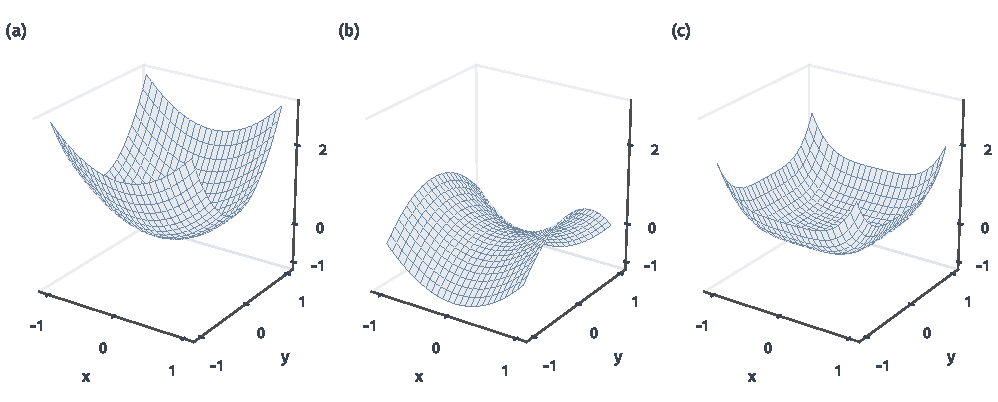
\includegraphics[width=169.0mm]{figures/01-mathematical-preliminaries-upper/01-mathematical-language-combinatorics-analysis-optimization/matplotlib/chapter3-concept-processes/hessian-local-shapes.pdf}
 \caption{同一$[-1,1]^2$范围和纵轴尺度下，三面分别为$x^2+2y^2$、$x^2-y^2$、$x^4+y^4$。原点的Hessian依次为正定、不定、零矩阵；前两者给严格极小与鞍点，第三者虽严格极小却不能由正定判据推出。零Hessian也可能没有极值，例如前述$x^3$，故退化不是一种确定分类。}
 \label{fig:analysis-process-hessian-local-shapes}
\end{figure*}

\FloatBarrier

\subsection{多元向量值函数的微分}

前面每个输入只产生一个实数。现在固定$F:U\subseteq\mathbb R^d\to\mathbb R^m$，同一输入同时产生$m$个输出分量；参数曲线与曲面也是这种映射的特殊情况。
有限个输出可以逐分量检查，但输入仍要整体扰动，不能以坐标切片代替各分量的全微分。

\subsubsection{向量值函数及其极限与连续性}

给出所有输出分量，就确定了整个映射；因此先按输出分量组织其表示。
\begin{definition}[多元向量值函数]
\label{def:multivariable-vector-function}
映射$F:U\subseteq\mathbb R^d\to\mathbb R^m$称为多元向量值函数，写作$F=(F_1,\ldots,F_m)^\top$，其中每个$F_i:U\to\mathbb R$为多元标量函数。
\end{definition}
其极限与连续性使用输出欧氏距离$\lVert F(\bm x)-\bm b\rVert_2$。
对有限个输出，这等价于每个$F_i$的对应极限存在或在同一基点连续，因为
\[
 \max_i|F_i(\bm x)-b_i|\leq\lVert F(\bm x)-\bm b\rVert_2
 \leq\sqrt m\max_i|F_i(\bm x)-b_i|.
\]
这里分解的是输出分量，区别于只沿某些输入坐标检查的切片。

\subsubsection{微分与Jacobian矩阵}

标量输出使用到实数的线性映射，也称线性泛函；向量输出则需要把输入扰动映射为$m$维输出扰动。
有限维线性映射由矩阵表示，矩阵的每一行记录一个输出分量的系数。
\begin{definition}[向量值函数的微分]
\label{def:multivariable-vector-differential}
设$U$开，$F:U\to\mathbb R^m$，$\bm a\in U$。若存在矩阵$\bm J_F(\bm a)\in\mathbb R^{m\times d}$，使
\begin{equation}
 F(\bm a+\bm h)=F(\bm a)+\bm J_F(\bm a)\bm h+o(\lVert\bm h\rVert_2),
\label{eq:analysis-jacobian-linearization}
\end{equation}
则称$F$在$\bm a$处可微，余项按输出欧氏范数理解。
其微分为$\mathrm dF_{\bm a}(\bm h)=\bm J_F(\bm a)\bm h$，其中$\bm J_F$称为\term{Jacobian矩阵}（Jacobian matrix），第$i,j$个元素为$\partial_jF_i$。
\end{definition}
向量值函数可微当且仅当每个输出分量$F_i$可微：正向可从向量余项取分量，反向则将有限个分量的$o(\lVert\bm h\rVert_2)$余项用欧氏范数合并。
因此Jacobian的第$i$行是标量分量梯度$\nabla F_i^\top$；$m=1$时Jacobian是梯度的转置，而不是梯度列向量本身。
$C^k$向量值函数指所有输出分量都属于$C^k$。


图~\ref{fig:analysis-process-jacobian-grid-cell}把向量值映射的线性近似画成小网格块的变化。后面区域换元还会使用这个局部矩阵的行列式。
\begin{figure*}[!htbp]
 \centering
 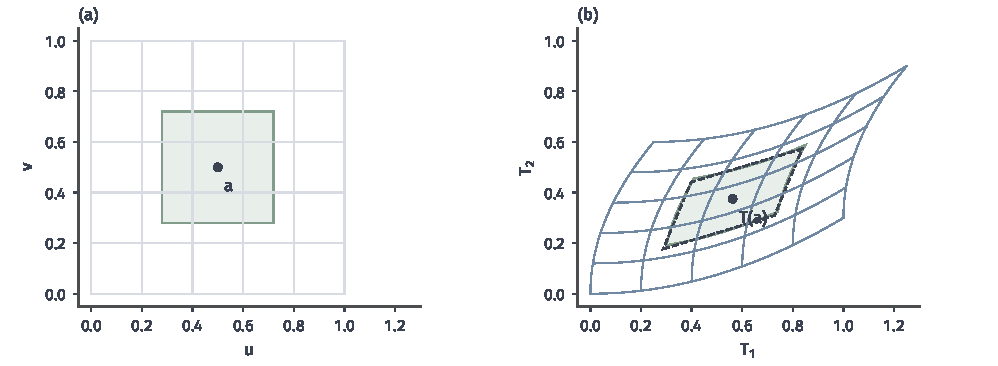
\includegraphics[width=169.0mm]{figures/01-mathematical-preliminaries-upper/01-mathematical-language-combinatorics-analysis-optimization/matplotlib/chapter3-concept-processes/jacobian-grid-cell.pdf}
 \caption{取$T(u,v)=(u+v^2/4,\,0.6v+0.3u^2)$，$a=(0.5,0.5)$。(a) 输入网格及绿色小方块。(b) 非线性像为弯边块，黑虚线为$T(a)+J_T(a)(h,k)^\top$给出的平行四边形；$J_T(a)=\bigl[\begin{smallmatrix}1&0.25\\0.3&0.6\end{smallmatrix}\bigr]$。有限块不与线性像完全重合，缩小扰动后才由可微余项控制差异。}
 \label{fig:analysis-process-jacobian-grid-cell}
\end{figure*}

\paragraph{Jacobian矩阵的计算}
每个输出先按标量函数求偏导，再按行排列，可以核对输入、输出与矩阵形状是否一致。
例如$F(x,y)=(x^2+xy,y^2)^\top$的Jacobian为
\[
 \bm J_F(x,y)=\begin{bmatrix}2x+y&x\\0&2y\end{bmatrix}.
\]
在$(1,2)$处，它把扰动$(h,k)^\top$的一阶影响写成$(4h+k,4k)^\top$。两个输出分别占一行，两个输入分别占一列。

若要把任意实数组变成正数且总和为$1$的权重，可以先取指数再除以共同的总和。
这就是$n$维\term{归一化指数映射}（softmax）。对正整数$n$和
$\bm{z}\in\mathbb{R}^n$，令
\[
  s_i(\bm{z})
  =
  \frac{e^{z_i}}{\sum_{k=1}^n e^{z_k}},
  \qquad i=1,\ldots,n.
\]
记分母为$Z=\sum_k e^{z_k}$。指数函数求导和商法则给出
\[
  \frac{\partial s_i}{\partial z_j}
  =
  \frac{\mathbb{I}\{i=j\}e^{z_i}Z-e^{z_i}e^{z_j}}{Z^2}
  =
  s_i\bigl(\mathbb{I}\{i=j\}-s_j\bigr).
\]
因此整个Jacobian矩阵为
\begin{equation}
  \bm{J}_{\bm{s}}(\bm{z})
  =
  \operatorname{diag}(\bm{s})-\bm{s}\bm{s}^{\top}.
\label{eq:analysis-softmax-jacobian}
\end{equation}
这里$\operatorname{diag}(\bm s)$表示以$s_1,\ldots,s_n$为对角元、其他元素为零的对角矩阵。
对角项$s_i(1-s_i)$描述提高$z_i$对自身分量的影响，非对角项$-s_is_j$
来自共同分母：提高一个坐标会压低其余归一化分量。每行元素之和为零，
这也与给所有$z_i$同时加同一常数不改变输出相符。



\subsubsection{向量值函数的微分运算}
\label{sec:analysis-vector-chain-matrix-calculus}

运算必须先有定义。相同形状的向量输出可以相加、相减和数乘；复合则要求前一映射的输出属于后一映射的定义域。
这里不把没有指定乘法含义的两个向量直接套入标量乘积法则。

\paragraph{和的微分}
若$F,H:U\to\mathbb R^m$在$\bm a$处可微，则逐分量使用和法则，得到
\[
 \bm J_{F+H}(\bm a)=\bm J_F(\bm a)+\bm J_H(\bm a).
\]
相加的输出形状以及两个Jacobian的形状必须分别一致。

\paragraph{差的微分}
在相同条件下，逐分量使用差法则，得到
\[
 \bm J_{F-H}(\bm a)=\bm J_F(\bm a)-\bm J_H(\bm a).
\]

\paragraph{数乘的微分}
对固定实数$c$，逐分量使用数乘法则，得到
\[
 \bm J_{cF}(\bm a)=c\bm J_F(\bm a).
\]

\paragraph{复合函数的链式法则}
前一映射产生的输出扰动，还要经过后一映射的线性响应。
因此复合微分按实际计算顺序组合，Jacobian的乘法次序由输入与输出维度决定。
\begin{theorem}[向量值函数的链式法则]
\label{thm:multivariable-vector-chain-rule}
设$U\subseteq\mathbb R^d$、$V\subseteq\mathbb R^m$开，$F:U\to V$在$\bm a$处可微，$G:V\to\mathbb R^p$在$F(\bm a)$处可微，则$G\circ F$在$\bm a$处可微，且
\begin{equation}
 \bm J_{G\circ F}(\bm a)=\bm J_G(F(\bm a))\bm J_F(\bm a).
\label{eq:analysis-vector-chain-rule}
\end{equation}
\end{theorem}
\begin{proof}
记$\bm A=\bm J_F(\bm a)$、$\bm B=\bm J_G(F(\bm a))$，由$F$可微有$\bm k=F(\bm a+\bm h)-F(\bm a)=\bm A\bm h+o(\lVert\bm h\rVert_2)$，故$\lVert\bm k\rVert_2=O(\lVert\bm h\rVert_2)$。
代入$G$的一阶展开得到$G(F(\bm a)+\bm k)-G(F(\bm a))=\bm B\bm A\bm h+o(\lVert\bm h\rVert_2)$，其中外层余项$o(\lVert\bm k\rVert_2)$也被原扰动尺度控制。
这正是复合函数的可微定义。
\end{proof}
矩阵形状为$(p\times m)(m\times d)=p\times d$，反向相乘往往没有定义。
即使两个次序都有定义，矩阵乘法一般也不交换，不能按标量经验调换因子。这项复合规则称为\term{链式法则}（chain rule）。

\paragraph{标量复合函数的梯度}

前面的外层映射$G$允许向量输出。当$p=1$时，它把中间向量变成一个标量。在优化问题中，
这个标量通常是待最小化的目标值，本书便把此时的$G$记为$\ell$。令
$\bm y=F(\bm x)$，总目标就是$L(\bm x)=\ell(F(\bm x))$；$\ell$只是原复合映射的
最后一层，并没有增加一个未说明的输出。采用列向量梯度，链式法则写成
\[
  \nabla L(\bm x)
  =\bm J_F(\bm x)^\top\nabla\ell(\bm y)\big|_{\bm y=F(\bm x)}.
\]
局部线性映射在前向计算中按$\bm J_F$作用，在标量目标的反向计算中按转置
$\bm J_F^\top$传回。这说明列向量梯度在复合时为何出现Jacobian的转置。


图~\ref{fig:analysis-process-chain-rule-types}把前向的函数复合与反向的梯度传递分开，便于核对转置及维度。
\begin{figure}[!htbp]
 \centering
 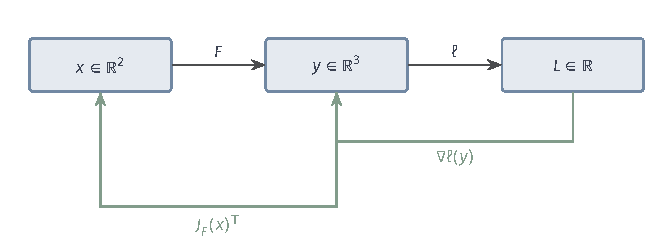
\includegraphics[width=112mm]{figures/01-mathematical-preliminaries-upper/01-mathematical-language-combinatorics-analysis-optimization/tikz/chapter3-concept-processes/chain-rule-types.pdf}
 \caption{上方是$x\in\mathbb R^2$经$F$产生$y\in\mathbb R^3$，再经$\ell$产生标量$L$。下方先得到$\nabla\ell(y)\in\mathbb R^3$，再由$2\times3$矩阵$J_F(x)^\top$传回$\nabla L(x)\in\mathbb R^2$。反向箭头表示梯度的线性传递，不表示对$F$或$\ell$求逆函数。}
 \label{fig:analysis-process-chain-rule-types}
\end{figure}

\begin{example}[从中间向量求回复合目标的梯度]
\label{ex:analysis-chain-rule-calculation}
令
\[
  F(x_1,x_2)=(x_1^2,x_1x_2,x_2)^\top,
  \qquad \ell(\bm y)=\frac12(y_1^2+y_2^2+y_3^2).
\]
$F$从二维输入产生三维中间量，$\ell$再把三维中间量变成一个数。于是
\[
  \bm J_F=\begin{bmatrix}2x_1&0\\x_2&x_1\\0&1\end{bmatrix},
  \qquad \nabla\ell(\bm y)=\bm y.
\]
在$\bm x=(1,2)^\top$处，$\bm y=(1,2,2)^\top$，链式法则给出
\[
  \nabla L(1,2)
  =\begin{bmatrix}2&2&0\\0&1&1\end{bmatrix}
    \begin{bmatrix}1\\2\\2\end{bmatrix}
  =\begin{bmatrix}6\\4\end{bmatrix}.
\]
也可以把复合函数直接展开为
$L(x_1,x_2)=\tfrac12(x_1^4+x_1^2x_2^2+x_2^2)$，求偏导得到
$\nabla L=(2x_1^3+x_1x_2^2,\,x_1^2x_2+x_2)^\top$，在同一点仍为$(6,4)^\top$。
两种计算处理同一个目标；链式形式保留了中间映射，可分别复用各层的导数。
矩阵形状$(2\times3)(3\times1)=2\times1$也核对了梯度传递的次序。
\end{example}


\subsubsection{向量增量的中值估计}

各输出分量的一元中值位置可能不同，不能保证有一个共同位置代表整个向量增量。
可以改为控制增量的范数，用线性映射的最大放大倍数估计有限变化。

\paragraph{算子范数}

对向量输出，用线性映射的最大放大倍数替代标量导数的绝对值。
\begin{definition}[欧氏诱导算子范数]
\label{def:analysis-induced-operator-norm}
对矩阵
$\bm{A}\in\mathbb{R}^{s\times r}$，由欧氏范数\term{诱导的算子范数}
（induced operator norm）定义为
\[
  \lVert\bm{A}\rVert_{\mathrm{op}}
  =
  \sup_{\bm{h}\neq\bm{0}}
  \frac{\lVert\bm{A}\bm{h}\rVert_2}{\lVert\bm{h}\rVert_2}
  =
  \sup_{\lVert\bm{h}\rVert_2=1}\lVert\bm{A}\bm{h}\rVert_2.
\]
\end{definition}
它表示线性映射对向量长度的最大放大倍数，定义立即给出
$\lVert\bm{A}\bm{h}\rVert_2
\leq\lVert\bm{A}\rVert_{\mathrm{op}}\lVert\bm{h}\rVert_2$。
例如$\bm A=\operatorname{diag}(2,1)$把第一坐标放大两倍、第二坐标保持不变，
故$\lVert\bm A\rVert_{\mathrm{op}}=2$；最大放大由第一坐标方向达到。

在含整条线段的开邻域内连续可微时，下面的范数界不要求各分量共用一个中值点。
\begin{theorem}[向量值函数的中值估计]
\label{thm:multivariable-vector-mean-value}
设$U\subseteq\mathbb R^r$开，$G:U\to\mathbb R^s$连续可微，且$[\bm y',\bm y]\subset U$，则
\begin{equation}
  \begin{aligned}
  \lVert G(\bm{y})-G(\bm{y}')\rVert_2
  &\leq
  \sup_{0\leq t\leq1}
  \left\lVert
    \bm{D}G\bigl(\bm{y}'+t(\bm{y}-\bm{y}')\bigr)
  \right\rVert_{\mathrm{op}}
  \lVert\bm{y}-\bm{y}'\rVert_2.
  \end{aligned}
\label{eq:analysis-operator-mean-value-bound}
\end{equation}
其中$\bm DG=\bm J_G$，即$G$的Jacobian矩阵。
\end{theorem}
\begin{proof}
这个向量上界无需预先使用积分公式。若$\bm u=G(\bm y)-G(\bm y')\neq\bm0$，
取单位向量$\bm v=\bm u/\lVert\bm u\rVert_2$，并沿线段定义标量函数
$\phi(t)=\bm v^\top G(\bm y'+t(\bm y-\bm y'))$。
中值定理给出某个$\tau\in(0,1)$，使
\[
 \lVert\bm u\rVert_2
 =\phi(1)-\phi(0)
 =\bm v^\top\bm DG(\bm y'+\tau(\bm y-\bm y'))(\bm y-\bm y').
\]
对右侧使用欧氏内积与算子范数的上界便得到式~\eqref{eq:analysis-operator-mean-value-bound}；
$\bm u=\bm0$时该界直接成立。
\end{proof}
若定义域为凸开集，且Jacobian的算子范数在全域不超过同一个有限$L$，则$G$为Lipschitz连续；局部球上的界给出局部版本。
特别地，若在某邻域内$L<1$，映射严格缩小任意两点间的距离。后面的隐函数构造将使用这一条件和几何尾和控制迭代。

\subsection{矩阵自变量函数的微分}

本小节的定义域$\mathcal U$均为全矩阵空间$\mathbb R^{m\times n}$中的开集，基点$\bm X\in\mathcal U$；因此全部充分小的同形扰动都允许使用。矩阵$\bm X$可以看成$mn$个实数坐标组成的输入；保留矩阵形状，能让乘法次序与迹的结构更清楚。
输出仍须分别说明：$f(\bm X)$为标量时使用矩阵梯度，$\Phi(\bm X)$为矩阵时则使用矩阵到矩阵的线性微分。

\subsubsection{矩阵标量函数的微分与梯度}

第~\ref{sec:prelim-matrix-trace}节已定义Frobenius内积与范数，满足$\langle\bm A,\bm B\rangle_F=\operatorname{tr}(\bm A^\top\bm B)$。
现在用该范数度量输入扰动，用该内积表示标量输出的一阶变化。
\begin{definition}[矩阵标量函数的梯度]
\label{def:multivariable-matrix-scalar-gradient}
设$f:\mathcal U\to\mathbb R$。若它在矩阵$\bm X$处满足
\[
 f(\bm X+\bm H)=f(\bm X)+\mathrm df_{\bm X}(\bm H)+o(\lVert\bm H\rVert_F),
\]
其中$\mathrm df_{\bm X}$为矩阵到实数的线性映射，则称$f$在该点可微。
唯一满足
\begin{equation}
 \mathrm df_{\bm X}(\bm H)=\langle\nabla_{\bm X}f,\bm H\rangle_F
 =\operatorname{tr}\bigl((\nabla_{\bm X}f)^\top\bm H\bigr)
\label{eq:analysis-matrix-gradient-definition}
\end{equation}
的同形矩阵$\nabla_{\bm X}f\in\mathbb R^{m\times n}$称为矩阵梯度。
\end{definition}
它的各元素是对相应矩阵坐标的偏导数，唯一性可逐个取只有一个非零元素的扰动检验。
计算时先用乘积法则展开微分，再利用迹的循环移位将扰动移到末端。例如乘积形状相容时，
\[
 \operatorname{tr}(\bm A\bm B)=\operatorname{tr}(\bm B\bm A),\qquad
 \operatorname{tr}(\bm A\bm B\bm C)=\operatorname{tr}(\bm B\bm C\bm A).
\]
这里循环移动的是整个因子，不能任意交换相邻矩阵。矩阵梯度的唯一性使用了全部矩阵方向；若把定义域限制在对称矩阵等子空间上，还需另行说明所用的内积与允许方向。

\paragraph{迹函数的微分}
线性迹函数已经符合定义，可以直接读出梯度。
对固定的$\bm{A}\in\mathbb{R}^{m\times n}$，令 $f(\bm{X})=\operatorname{tr}(\bm{A}^{\top}\bm{X})$。它的微分已经符合式
\eqref{eq:analysis-matrix-gradient-definition}，所以
\begin{equation}
  \nabla_{\bm{X}}\operatorname{tr}(\bm{A}^{\top}\bm{X})
  =\bm{A}.
\label{eq:analysis-trace-linear-gradient}
\end{equation}
这个简单关系常用于从迹表达式中读出梯度。

\paragraph{行列式的微分}
行列式把方阵映为一个实数，可以通过有限多项式展开来求微分。下面先在可逆矩阵处计算，便于使用行列式的乘法公式。
第~\ref{sec:prelim-determinants}节的有限多项式表达式可用来直接识别一阶项。
先设$\bm X\in\mathbb R^{d\times d}$可逆。
计算它的一阶变化，先把方向扰动$\bm H$从行列式中分离出来：
\[
 \det(\bm X+t\bm H)=\det(\bm X)\det(\bm I+t\bm X^{-1}\bm H).
\]
对固定矩阵$\bm B$，行列式的排列展开给出
$\det(\bm I+t\bm B)=1+t\operatorname{tr}(\bm B)+O(t^2)$。
其中一次项只能从恒等排列的一个对角位置选取$tB_{i,i}$，其余位置选$1$；
非恒等排列至少改变两个位置，因此只贡献二次及以上项。
行列式是有限多项式，故在固定$\bm X$附近，对任意小矩阵扰动$\bm H$，
同一展开中的二阶及更高阶项也统一为$O(\lVert\bm H\rVert_F^2)$；这保证得到的是全微分，而不只是固定方向上的导数。
代入$\bm B=\bm X^{-1}\bm H$，便得到Jacobi行列式公式的一阶形式
\[   \mathrm{d}\det\bm{X}   =   \det(\bm{X})\operatorname{tr}   (\bm{X}^{-1}\mathrm{d}\bm{X}). \]
\paragraph{对数行列式的微分}
实数对数还要求$\det\bm X>0$，它在该开集上与行列式复合。对上面的微分应用标量对数的链式法则，得到
\begin{equation}
  \mathrm{d}\log\det\bm{X}
  =
  \operatorname{tr}(\bm{X}^{-1}\mathrm{d}\bm{X}),
  \qquad
  \nabla_{\bm{X}}\log\det\bm{X}
  =
  \bm{X}^{-\top}.
\label{eq:analysis-logdet-gradient}
\end{equation}
若$\bm X$还对称，则$\bm{X}^{-\top}=\bm{X}^{-1}$；一般情形应保留转置。
这些计算都先找出扰动的一阶项，再用迹内积读出梯度；乘积次序与行列式展开决定了哪些变形成立。

\subsubsection{矩阵值函数的微分}

求逆映射的输出与输入都是方阵，不能用一个同形梯度表示全部输出的一阶变化。
若$\Phi:\mathcal U\to\mathbb R^{r\times s}$满足$\Phi(\bm X+\bm H)=\Phi(\bm X)+A(\bm H)+o(\lVert\bm H\rVert_F)$，其中$A$为矩阵空间之间的线性映射、余项按输出Frobenius范数度量，则$A$为其微分。
这就是前面的向量值可微性按矩阵形状重排，不能把不同输出元素共用一个标量系数。

\paragraph{逆矩阵的微分}
逆矩阵与行列式非零的关系在第~\ref{sec:prelim-inverse-matrices}节及第~\ref{sec:prelim-determinants}节已经建立。
这里先确认可微，再对乘法恒等式取微分。
第~\ref{sec:prelim-determinants}节的代数余子式公式把逆矩阵的各元素写成多项式与$\det\bm X$的比。
因此，在$\det\bm X\neq0$的开集内，每个元素都是连续可微函数，逆映射也连续可微。
确认可微性后，对恒等式$\bm{X}\bm{X}^{-1}=\bm{I}$取微分可得
\[   (\mathrm{d}\bm{X})\bm{X}^{-1}   +\bm{X}\,\mathrm{d}(\bm{X}^{-1})=\bm{0}. \]
左乘$\bm{X}^{-1}$后得到
\begin{equation}
  \mathrm{d}(\bm{X}^{-1})
  =
  -\bm{X}^{-1}(\mathrm{d}\bm{X})\bm{X}^{-1}.
\label{eq:analysis-inverse-differential}
\end{equation}
两个$\bm{X}^{-1}$位于扰动两侧，不能合并成 $-\bm{X}^{-2}\mathrm{d}\bm{X}$，因为$\mathrm{d}\bm{X}$未必与$\bm{X}^{-1}$交换。



\begin{example}[逆矩阵微分中的乘法次序]
\label{ex:analysis-noncommuting-inverse-differential}
取$\bm X=\operatorname{diag}(2,1)$，扰动方向
$\bm E=\begin{bmatrix}0&1\\1&0\end{bmatrix}$。沿$\bm X+t\bm E$求逆矩阵的导数为
\[
 -\bm X^{-1}\bm E\bm X^{-1}
 =\begin{bmatrix}0&-1/2\\-1/2&0\end{bmatrix}.
\]
若照搬标量规则而写成$-\bm X^{-2}\bm E$，会得到
$\begin{bmatrix}0&-1/4\\-1&0\end{bmatrix}$，连对称性都丢失。
原路径在$0$附近由对称可逆矩阵组成，其逆与导数也应对称；这一结构检查能直接发现错误。
矩阵变量沿给定方向微分时，夹在两侧的逆矩阵不能随意移到同一侧。
\end{example}

\subsection{隐函数与反函数}
\label{sec:analysis-implicit-parameter-integral}

前面把已给定的映射作微分；这里改变问题，先给定一组方程，再判断它是否在基点附近确定唯一的函数。
一般方程组采用向量值映射，待解变量与方程数量的对应关系决定哪个Jacobian必须可逆。

\subsubsection{隐函数的定义}

显式函数直接给出输出，例如$y=\sqrt x$。关系$F(x,y)=0$则没有直接选定一个输出。
若在一点$(a,b)$附近存在函数$y=\varphi(x)$，使这些局部解恰好满足$y=\varphi(x)$，就称方程在此确定了一个\term{隐函数}（implicit function）。
隐函数研究的第一步是局部解分支存在且唯一，然后才是对这条分支求导。

例如方程$y^2-x=0$在$x>0$时有正、负两支解。固定其中一个非零解后，可以在它附近选出唯一分支；但在$(0,0)$，两支相交，负$x$侧还没有实数解，因此不存在覆盖$0$的开区间上的可微解函数。此处$\partial F/\partial y=2y=0$，恰好失去了下面定理要求的可逆性。这个例子说明，局部选解既要指定起始解，也要核对关于待解变量的导数。

图~\ref{fig:vol1-add-implicit-branches}说明“局部唯一”怎样排除另一支解。在$(1,1)$附近只保留正支即可；在原点处，两支相交且负$x$没有实数解，不能沿用同样的局部可微选解。
\begin{figure}[!htb]
  \centering
  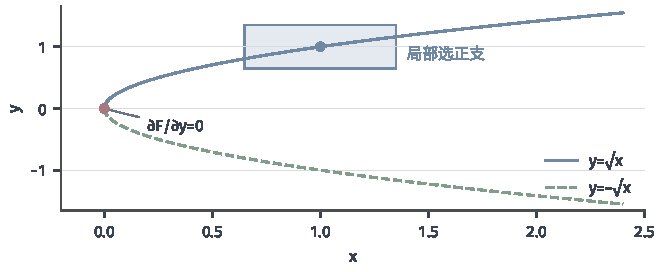
\includegraphics[width=112mm]{figures/01-mathematical-preliminaries-upper/01-mathematical-language-combinatorics-analysis-optimization/matplotlib/comprehension-additions/implicit-branches.pdf}
  \caption{方程$F(x,y)=y^2-x=0$的两支实数解。浅蓝矩形围住$(1,1)$，在该矩形内每个允许的$x$只有正支解，且$F_y=2y\neq0$；红点处$F_y=0$，两支相交。图的两个根都属于同一方程，选定起始解与邻域才确定隐函数分支。}
  \label{fig:vol1-add-implicit-branches}
\end{figure}
\FloatBarrier


\subsubsection{隐函数的存在、唯一性与微分}

下面的充分条件先保证局部解存在且唯一，再保证解随参数连续可微。
可逆性只要求待解变量对应的方阵Jacobian可逆，并非要求整个带参数映射为方阵。
\begin{theorem}[隐函数定理]
\label{thm:analysis-implicit-function}
设$F:\mathbb{R}^p\times\mathbb{R}^m\to\mathbb{R}^m$在 $(\bm{a},\bm{b})$的某个开邻域内连续可微， $F(\bm{a},\bm{b})=\bm{0}$，并且关于待解变量的Jacobian矩阵 \[   \bm{D}_{\bm{y}}F(\bm{a},\bm{b})   \in\mathbb{R}^{m\times m} \]
可逆。则存在$\bm{a}$与$\bm{b}$的邻域$U,V$，以及唯一的连续可微函数
$\varphi:U\to V$，使$\varphi(\bm{a})=\bm{b}$，并且对所有
$(\bm{x},\bm{y})\in U\times V$都有
\[
  F(\bm{x},\bm{y})=\bm{0}
  \quad\Longleftrightarrow\quad
  \bm{y}=\varphi(\bm{x}).
\]
其Jacobian矩阵满足
\begin{equation}
  \bm{D}\varphi(\bm{x})
  =
  -
  \bigl[\bm{D}_{\bm{y}}F(\bm{x},\varphi(\bm{x}))\bigr]^{-1}
  \bm{D}_{\bm{x}}F(\bm{x},\varphi(\bm{x})).
\label{eq:analysis-implicit-derivative}
\end{equation}
\end{theorem}

证明将方程改写为局部压缩迭代，再分别检查统一压缩、自映射与解的可微性；形式求导不能替代这些存在性步骤。
\begin{proof}
为证明定理~\ref{thm:analysis-implicit-function}的存在性，先把方程改写为局部压缩迭代。记
\[   \bm{A}   =   \bm{D}_{\bm{y}}F(\bm{a},\bm{b}),   \qquad   T_{\bm{x}}(\bm{y})   =   \bm{y}-\bm{A}^{-1}F(\bm{x},\bm{y}). \]
$F(\bm{x},\bm{y})=\bm{0}$当且仅当$T_{\bm{x}}(\bm{y})=\bm{y}$，即$\bm y$是更新后保持不变的点，称为不动点。并且
\[   \bm{D}_{\bm{y}}T_{\bm{x}}(\bm{y})   =   \bm{I}   -   \bm{A}^{-1}\bm{D}_{\bm{y}}F(\bm{x},\bm{y}), \]
它在$(\bm{a},\bm{b})$处为零。由导数连续性，可以选择闭球 $B=\{\bm{y}:\lVert\bm{y}-\bm{b}\rVert_2\leq r\}$和$\bm{a}$的邻域$U$，使
\begin{equation}
  \sup_{\bm{x}\in U,\,\bm{y}\in B}
  \left\lVert
    \bm{D}_{\bm{y}}T_{\bm{x}}(\bm{y})
  \right\rVert_{\mathrm{op}}
  \leq q<1.
\label{eq:analysis-ift-uniform-contraction}
\end{equation}
沿$\bm{y}$方向使用式~\eqref{eq:analysis-operator-mean-value-bound}可知，每个
$T_{\bm{x}}$都把$B$内任意两点之间的距离缩小到原来的至多$q$倍。

还必须核对自映射。因为$T_{\bm{a}}(\bm{b})=\bm{b}$且$T_{\bm{x}}(\bm{b})$关于 $\bm{x}$连续，可进一步缩小$U$，使
\[   \lVert T_{\bm{x}}(\bm{b})-\bm{b}\rVert_2   \leq\frac{1-q}{2}r. \]
于是对$\bm{y}\in B$，
\[
  \lVert T_{\bm{x}}(\bm{y})-\bm{b}\rVert_2
  \leq
  q\lVert\bm{y}-\bm{b}\rVert_2+\frac{1-q}{2}r
  \leq
  \frac{1+q}{2}r
  <r.
\]
所以$T_{\bm{x}}(B)$包含在$B$的内部$V$中。
固定$\bm x\in U$，从$\bm y_0=\bm b$出发，令$\bm y_{n+1}=T_{\bm x}(\bm y_n)$。
所有迭代项都留在$B$内，相邻差满足
$\lVert\bm y_{n+1}-\bm y_n\rVert_2\leq q^n\lVert\bm y_1-\bm y_0\rVert_2$。
增大$q$仍保留这个上界，因而可设$0<q<1$。对$m>n$，几何和给出
\[
 \lVert\bm y_m-\bm y_n\rVert_2
 \leq\sum_{j=n}^{m-1}\lVert\bm y_{j+1}-\bm y_j\rVert_2
 \leq\frac{q^n}{1-q}\lVert\bm y_1-\bm y_0\rVert_2\longrightarrow0.
\]
每个坐标都是实柯西列，所以该序列在有限维欧氏空间中收敛；闭性使极限仍在$B$内。
$T_{\bm x}$连续，令$n\to\infty$可得极限$\varphi(\bm x)$满足
$T_{\bm x}(\varphi(\bm x))=\varphi(\bm x)$，而映射的内部包含关系使它属于$V$。
若另有不动点$\bm z$，则
$\lVert\bm z-\varphi(\bm x)\rVert_2\leq q\lVert\bm z-\varphi(\bm x)\rVert_2$，
由$q<1$只能有$\bm z=\varphi(\bm x)$，所以这个不动点唯一。若
$(\bm{x},\bm{y})\in U\times V$且$F(\bm{x},\bm{y})=\bm{0}$，则$\bm{y}\in B$也是
$T_{\bm{x}}$的不动点，唯一性迫使$\bm{y}=\varphi(\bm{x})$。这证明了定理所述的局部
存在与零点集合的逐点唯一性。

还需说明所得解随参数连续可微。把$U$进一步缩小为开球，并使
$\overline U\times B$包含在原定义域内；这个集合闭且有界，关于$\bm x$的导数各分量连续，
故有统一范数上界$L$。对$\bm x,\bm x'\in U$，
两点间的线段仍在$U$内，式~\eqref{eq:analysis-operator-mean-value-bound}
可用于$T_{\bm x}(\bm y)$的参数变化。利用两个不动点关系，
\[   \lVert\varphi(\bm{x})-\varphi(\bm{x}')\rVert_2   \leq   q\lVert\varphi(\bm{x})-\varphi(\bm{x}')\rVert_2   +L\lVert\bm{x}-\bm{x}'\rVert_2, \]
移项得到$\lVert\varphi(\bm x)-\varphi(\bm x')\rVert_2
\leq L\lVert\bm x-\bm x'\rVert_2/(1-q)$，
故$\varphi$局部Lipschitz连续。令 $\bm{h}\to\bm{0}$并记 $\bm{k}=\varphi(\bm{x}+\bm{h})-\varphi(\bm{x})$，前述界给出 $\lVert\bm{k}\rVert_2=O(\lVert\bm{h}\rVert_2)$。对恒等式
\[   F(\bm{x}+\bm{h},\varphi(\bm{x})+\bm{k})   -   F(\bm{x},\varphi(\bm{x}))   =   \bm{0} \]
作一阶展开，得到
\[   \bm{D}_{\bm{x}}F\,\bm{h}   +   \bm{D}_{\bm{y}}F\,\bm{k}   +   o(\lVert\bm{h}\rVert_2)   =   \bm{0}. \]
展开中的Jacobian均在$(\bm x,\varphi(\bm x))$处取值，联合扰动的余项
$o(\lVert(\bm h,\bm k)\rVert_2)$因$\lVert\bm k\rVert_2=O(\lVert\bm h\rVert_2)$
成为$o(\lVert\bm h\rVert_2)$。
基点的$\det\bm A\neq0$，行列式又是矩阵元素的连续函数，
所以邻域足够小时$\bm D_{\bm y}F$仍可逆。于是
\[   \bm{k}   =   -   (\bm{D}_{\bm{y}}F)^{-1}   \bm{D}_{\bm{x}}F\,\bm{h}   +   o(\lVert\bm{h}\rVert_2). \]
这证明$\varphi$可微并给出式~\eqref{eq:analysis-implicit-derivative}；各Jacobian矩阵连续又保证$\bm{D}\varphi$连续。至此，隐函数定理中的存在、局部唯一与导数公式都已得到说明。证明中特别核对了自映射和统一压缩条件，只有形式上的固定点改写并不足够。
\end{proof}

\paragraph{隐函数的导数}

定理的证明已同时建立解分支的存在、唯一性、可微性及式~\eqref{eq:analysis-implicit-derivative}。计算时只需在选定分支上代入两个Jacobian；下面用最初的方程核对正、负分支各自的变化率。

\begin{example}[隐函数分支的导数]
设$F(x,y)=y^2-x$，在$(1,1)$处有$F=0$、$F_y=2\neq0$。
隐函数定理保证$(1,1)$附近的解可以唯一写成$y=\varphi(x)$，且
\[
 \varphi'(x)=-\frac{F_x(x,\varphi(x))}{F_y(x,\varphi(x))}
 =\frac1{2\varphi(x)},\qquad \varphi'(1)=\frac12.
\]
直接选正支$\varphi(x)=\sqrt x$，求导同样得到$1/(2\sqrt x)$。
若在$(1,-1)$附近选负支，导数则为$-1/2$；起始解不同，所追踪的函数也不同。
\end{example}


\subsubsection{反函数的存在与微分}

反求一个向量值映射的输入，可以看成以输出为参数的一组方程，从而回用隐函数的结论。
以下只保证邻域之间的逆，不预先断言整个定义域上的映射单射。
\begin{theorem}[局部反函数定理]
\label{thm:multivariable-inverse-function}
设$U\subseteq\mathbb R^d$开，$G:U\to\mathbb R^d$连续可微，$\bm a\in U$，且$\bm J_G(\bm a)$可逆。
则存在$\bm a$的开邻域$U_0$与$G(\bm a)$的开邻域$V_0$，使$G:U_0\to V_0$为双射，逆映射连续可微，并满足
\[
 \bm J_{G^{-1}}(G(\bm x))=[\bm J_G(\bm x)]^{-1}
 \qquad(\bm x\in U_0).
\]
\end{theorem}
\begin{proof}
以输出$\bm y$为参数、原输入$\bm x$为待解变量，令$H(\bm y,\bm x)=G(\bm x)-\bm y$。
在$(G(\bm a),\bm a)$处，关于$\bm x$的Jacobian就是可逆的$\bm J_G(\bm a)$。隐函数定理给出开邻域$V_0$、$W$以及$C^1$映射$\varphi:V_0\to W$，使
\[
 G(\bm x)=\bm y\quad\Longleftrightarrow\quad\bm x=\varphi(\bm y)
 \qquad(\bm y\in V_0,\ \bm x\in W).
\]
将$W$缩小并重新选取$V_0$，可使$W\subset U$且$\bm J_G$在$W$内均可逆。
令$U_0=W\cap G^{-1}(V_0)$，它因$G$连续而为包含$\bm a$的开集。
每个$\bm y\in V_0$都有$G(\varphi(\bm y))=\bm y$，故$\varphi(\bm y)\in U_0$；反之，每个$\bm x\in U_0$都由上述唯一性满足$\varphi(G(\bm x))=\bm x$。
因此$G:U_0\to V_0$为双射，逆就是$C^1$映射$\varphi$。
对$G(\varphi(\bm y))=\bm y$使用链式法则，得到$\bm J_G(\varphi(\bm y))\bm J_\varphi(\bm y)=\bm I$，左乘逆矩阵便得到所述公式。
\end{proof}

\paragraph{局部可逆与整体单射}

Jacobian处处可逆仍不保证整个定义域上单射。例如
$g(u,v)=(e^u\cos v,e^u\sin v)^\top$的Jacobian行列式为$e^{2u}>0$，
但$v$与$v+2\pi$给出同一输出。它在每一点附近可以反求，整个平面上的输入却会重复覆盖输出。
反过来，存在连续逆也不保证逆可微：一元函数$x\mapsto x^3$全局单射，
其逆在$0$处没有有限导数。使用局部逆定理时，需要逐项检查邻域、可微性和可逆Jacobian。

\FloatBarrier
